\documentclass{beamer}
\usepackage[utf8]{inputenc}

\usetheme{Madrid}
\usecolortheme{default}
\usepackage{amsmath,amssymb,amsfonts,amsthm}
\usepackage{txfonts}
\usepackage{multicol}
\usepackage{tkz-euclide}
\usepackage{listings}
\usepackage{adjustbox}
\usepackage{array}
\usepackage{tabularx}
\usepackage{gvv}
\usepackage{lmodern}
\usepackage{circuitikz}
\usepackage{tikz}
\usepackage{graphicx}
\usepackage{hyperref}

\setbeamertemplate{page number in head/foot}[totalframenumber]

\usepackage{tcolorbox}
\tcbuselibrary{minted,breakable,xparse,skins}



\definecolor{bg}{gray}{0.95}
\DeclareTCBListing{mintedbox}{O{}m!O{}}{%
  breakable=true,
  listing engine=minted,
  listing only,
  minted language=#2,
  minted style=default,
  minted options={%
    linenos,
    gobble=0,
    breaklines=true,
    breakafter=,,
    fontsize=\small,
    numbersep=8pt,
    #1},
  boxsep=0pt,
  left skip=0pt,
  right skip=0pt,
  left=25pt,
  right=0pt,
  top=3pt,
  bottom=3pt,
  arc=5pt,
  leftrule=0pt,
  rightrule=0pt,
  bottomrule=2pt,
  toprule=2pt,
  colback=bg,
  colframe=orange!70,
  enhanced,
  overlay={%
    \begin{tcbclipinterior}
    \fill[orange!20!white] (frame.south west) rectangle ([xshift=20pt]frame.north west);
    \end{tcbclipinterior}},
  #3,
}
\lstset{
    language=C,
    basicstyle=\ttfamily\small,
    keywordstyle=\color{blue},
    stringstyle=\color{orange},
    commentstyle=\color{green!60!black},
    numbers=left,
    numberstyle=\tiny\color{gray},
    breaklines=true,
    showstringspaces=false,
}
%------------------------------------------------------------
%This block of code defines the information to appear in the
%Title page
\title %optional
{4.5.6}
\date{September 12,2025}
%\subtitle{A short story}

\author % (optional)
{Aditya Appana - EE25BTECH11004}



\begin{document}


\frame{\titlepage}
\begin{frame}{Question}
Find the equations of the line that passes through the point (3,0,1) and parallel to the
planes $x + 2y = 0$ and $3y$ $-$ $z = 0$.
\end{frame}



\begin{frame}[fragile]
    \frametitle{Solution}

We know that the normal form of a plane is $\vec{n}^T\vec{x} = 0$ \\
The plane $x + 2y = 0$ can be expressed in vector form as:
\begin{align}
    \myvec{1\\2\\0}^T\vec{x} = 0
\end{align} 

therefore, \begin{align}\vec{n}_1 = \myvec{1\\2\\0}\end{align} \\
The plane $3y$ $-$ $z=0$ can be expressed in vector form as:

\begin{align}
    \myvec{0 \\ 3 \\-1}^T\vec{x} = 0
\end{align}
\end{frame}


\begin{frame}[fragile]
    \frametitle{Solution}
therefore, \begin{align}\vec{n}_2 = \myvec{0\\3\\-1} \end{align}

The vector parallel to both planes will be perpendicular to the normal vectors of both planes. Therefore it can be expressed as
\begin{align} \vec{n}_1 \times \vec{n}_2 \end{align}

To calculate the cross product of the two vectors \vec{a} and \vec{b}, we use the following determinant:
\begin{center}
\myvec{|\vec{A_{11}} \vec{B_{23}}| \\ |\vec{A_{11}}   \vec{B_{23}}| \\ |\vec{A_{11}} \vec{B_{23}}| }
\end{center}
Where \vec{X_{ij}} = \myvec{$x_i$ \\ $x_j$}.
\end{frame}

\begin{frame}[fragile]
    \frametitle{Solution}
Expanding the determinants, we get: \begin{align}
\myvec{ ((-2) - 0) \\ (1-0)  \\ (3-0))} = \myvec{-2\\1\\3} \end{align}\\ 

Since the line passes through (3,0,1), the line can therefore be expressed as: \\
\begin{align}
\frac{x-3}{-2} = \frac{y}{1} = \frac{z-1}{3}
\end{align} 
\end{frame}


\begin{frame}[fragile]
    \frametitle{Python, C, Python+C Codes}

\href{https://github.com/AdityaAppana/ee1030-2025/tree/8428703b12dd76c7f155f1738158e50a858c4817/ee25btech11004/matgeo/4.5.6/Codes}{codes permalink}

\end{frame}

\begin{frame}
\frametitle{Plot}
\begin{figure}[H]
    \centering
    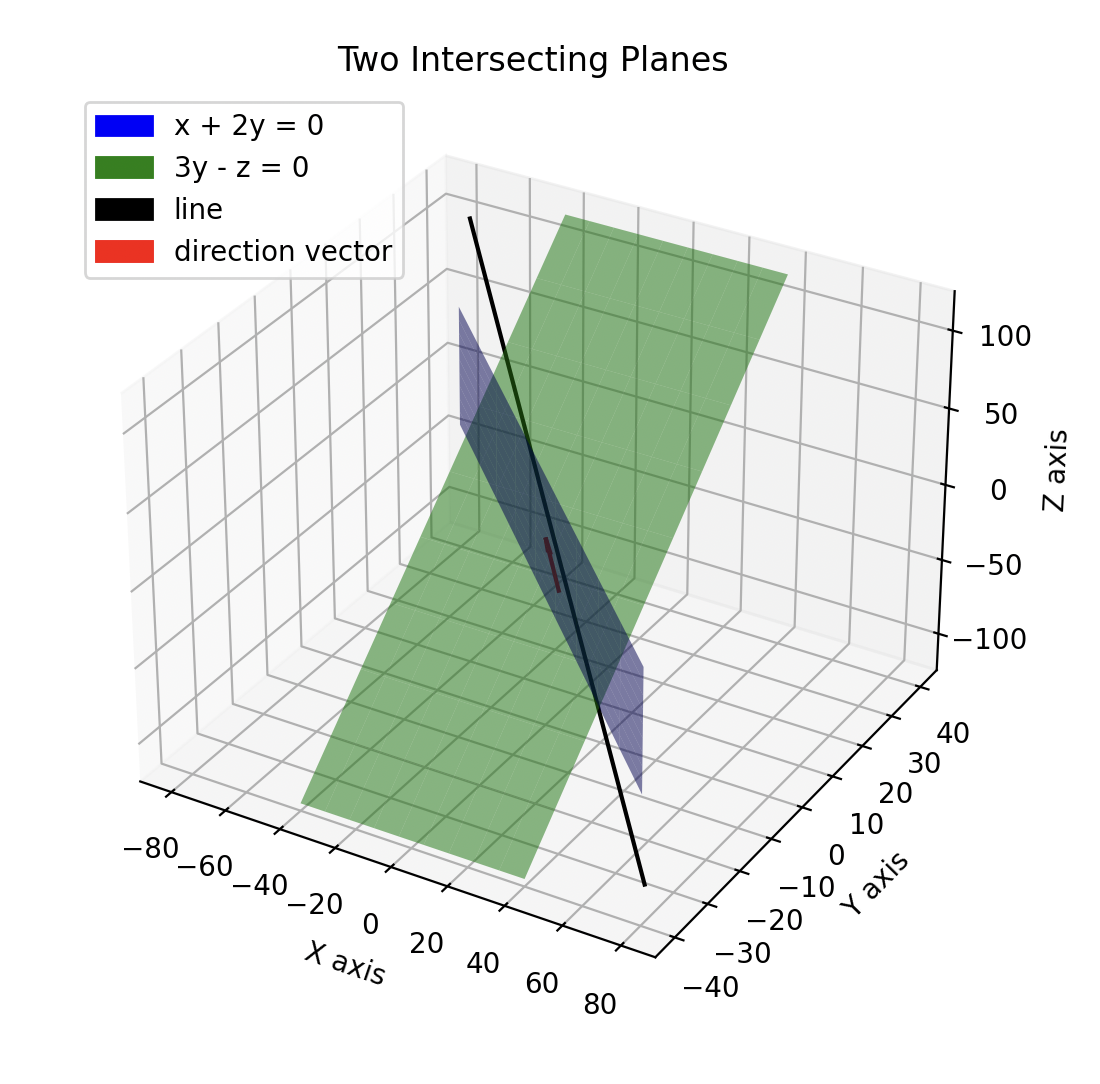
\includegraphics[width=0.6\columnwidth]{Figs/Plot7.png}
    \caption{Plot}
    \label{fig:placeholder}
\end{figure}

\end{frame}



\end{document}